\renewcommand{\theequation}{\theenumi}
\renewcommand{\thefigure}{\theenumi}
\renewcommand{\thetable}{\theenumi}
\begin{enumerate}[label=\thesection.\arabic*.,ref=\thesection.\theenumi]
\numberwithin{equation}{enumi}
\numberwithin{figure}{enumi}
\numberwithin{table}{enumi}


\item Let $X_n$ denote the sum of points obtained when n fair dice are rolled together. The expectation and variance of $X_n$ are

\begin{enumerate}
\begin{multicols}{2}
\setlength\itemsep{1em}
{\scriptsize
\item ${\dfrac{7}{2}}n$ and ${\dfrac{35}{12}}n^2$ respectively.
\item ${\dfrac{7}{2}}n$ and ${\dfrac{35}{12}}n$ respectively.
\item $ \bigg (\dfrac{7}{2} \bigg )^n$ and $ \bigg (\dfrac{35}{12} \bigg )^n$ respectively.
\item None of the above
}
\end{multicols}
\end{enumerate}
\solution
We know, when one dice is rolled probability i.e \pr{X_{1}=r} for all r in \{1,2,3,4,5,6\} is equal to  p
\begin{align}
    p&=\frac{1}{6}
\end{align}
Let $Y_{i}$ denote the value obtained on ith dice when n dices are rolled  
, therefore 
\begin{align}
  X_{n}&=\sum_{i=1}^n Y_{i}
  \label{ec64:eq:eq1}
\end{align}
Now i will calculate expectation value of value obtained when one dice is rolled
using below formula;
\begin{align}
 E(Y_{i})&= E( X_{1}) =\sum_{r=1}^6 (r\times p)
 \label{ec64:eq:eq2}
\\
&=\frac{1}{6} \times \sum_{r=1}^6 r
\\
&=\frac{7}{2}.
\label{ec64:eq:eq3}
\end{align}
\begin{enumerate}
\item Since the Expectation value of a sum of independent events is the sum of their expectation. So,
\begin{align}
    E(X_{n})&=\sum_{i=1}^n E(Y_{i})
    \\
    & = \sum_{i=1}^n \frac{7}{2} =\frac{7}{2} n 
\label{ec64:eq:eq4}
\end{align}
\item By Using the following formula ,we can calculate variance of  $X_{1}$ ,
\begin{align}
    V(X_{1})&=(E(X_{1})^{2}) - (E(X_{1}))^{2}
    \label{ec64:eq:eq5}
    \\
    \sum_{i=1}^k r^2&=\frac{k\times (k+1 )\times (2(k)+1)}{6}
    \label{ec64:eq:eq6}
\end{align}
Now calculating E($X_{1}^{2}$),by using \eqref{ec64:eq:eq6}
\begin{align}
    E(X_{1}^{2})&=\sum_{r=1}^6(r^{2}\times p)
    \\
    &=\frac{1}{6}\times\sum_{r=1}^6r^{2}
    \\
    &=\frac{91}{6}
    \label{ec64:eq:eq7}
\end{align}
By using \eqref{ec64:eq:eq3},\eqref{ec64:eq:eq5} and \eqref{ec64:eq:eq7}
\begin{align}
    V(X_{1})&=V(Y_{i})
    \\
    &=\frac{35}{12}
    \label{ec64:eq:eq8}
\end{align}
Variance of sum can be calculated by using following formula,
\begin{align}
    V(X_{n})&=V(\sum_{i=0}^n Y_{i})
    \\
    &= \sum_{i=1}^n V(Y_{i}) + \sum_{1\leq i\not=j \leq n}\text{Cov}(Y_{i},Y_{j})
\end{align}
Since Co-variance of independent random variables is zero.So,
\begin{align}
    V(X_{n})&=\sum_{i=1}^n V(Y_{i}) + 0
    \\
    &=\frac{35}{12}n
\end{align}
\end{enumerate}
    Hence option(B) is correct.

%
\item
Consider that X and Y are independent continuous valued random variables with uniform PDF given by $X\sim U(2,3)$ and $Y\sim U(1,4)$. Then $\pr{Y\le X}$ is equal to .....
\\
\solution

\begin{figure}[!ht]
\centering
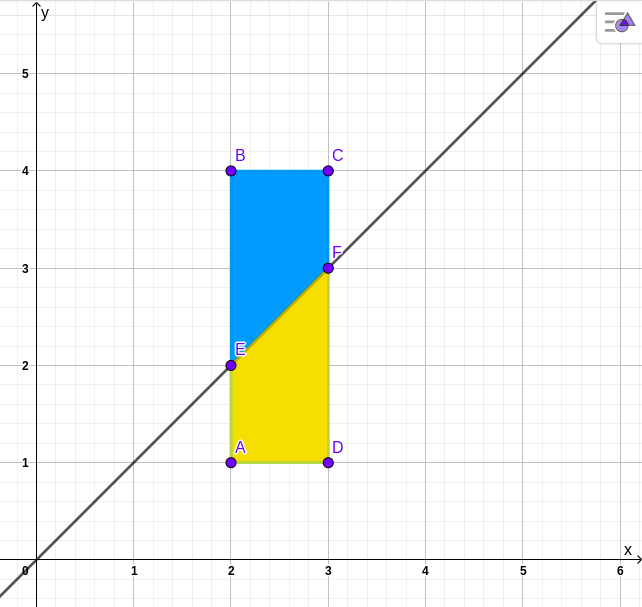
\includegraphics[width=\columnwidth]{solutions/in/2021/figures/figure.png}
\caption{Probability Distribution of (X, Y)}
\label{fig:Nuruhuhuhuhuhuhu}
\end{figure}

In figure \ref{fig:Nuruhuhuhuhuhuhu}, rectangle ABCD represents sample space of (X, Y). $Y \le X$ for any point (X, Y) if and only if the point lies on or below line EF. Therefore 
\begin{align}
    \pr{Y \le X} = \cfrac{Area\; of\; AEFD}{Area\; of\; ABCD}\\
                 = \cfrac{1}{2}    
\end{align}

Alternately, we have PDF and CDF of X and Y given by 
\begin{align}
    f_X(x) = 
    \begin{cases}
    1 & 2\le x\le 3\\
    0 & otherwise
    \end{cases}
\end{align}
\begin{align}
    F_X(x) = 
    \begin{cases}
    0   & x < 2\\
    x-2 & 2\le x\le 3\\
    1   & x > 3
    \end{cases}
\end{align}
\begin{align}
    f_Y(x) = 
    \begin{cases}
    1 & 1\le x\le 4\\
    0 & otherwise
    \end{cases}
\end{align}
\begin{align}
    F_Y(x) = 
    \begin{cases}
    0   & x < 1\\
    \cfrac{x-1}{3} & 1\le x\le 4\\
    1   & x > 4
    \end{cases}
\end{align}
Thus 
\begin{align}
    \pr{Y\le X} &= \int_{-\infty}^{\infty} F_Y(x)f_X(x)dx\\
                &= \int_2^3 \cfrac{x-1}{3}dx\\
                &= \cfrac{1}{2}
\end{align}



%

%
\item Given Set A = \{2,3,4,5\} and Set B = \{11,12,13,14,15\}, two numbers are randomly selected, one from each set. What is probability that the sum of the two numbers equals 16?
\\
%
\solution

Let $X_1\in\,$\cbrak{2,3,4,5} and $X_2\in\,$\cbrak{11,12,13,14,15} be the random variables such that $X_1$ represents the number chosen from set A and $X_2$ the number chosen from set B.\\
Then, the probability mass functions are 
\begin{align}
    p_{X_1}(n) = \pr{X_1 = n} = 
    \begin{cases}
    \frac{1}{4} & 2 \leq n \leq 5\\
    0 & otherwise
\end{cases}\label{ee2015-2:1}
\end{align}
\begin{align}
    p_{X_2}(n) = \pr{X_2 = n} = 
    \begin{cases}
    \frac{1}{5} & 11 \leq n \leq 15\\
    0 & otherwise
\end{cases}\label{ee2015-2:2}
\end{align}
Let X be the random variable denoting the sum (X=$X_1$+$X_2$). Then, X can take the values \cbrak{13,14,15,16,17,18,19,20}.
\begin{align}
     p_X(n)&=\pr{X_1+X_2=n}\\
     &=\pr{X_1=n-X_2}\\
     &=\Sigma_{k}{\pr{X_1=n-k|X_2=k}p_{X_2}(k)}\label{ee2015-2:3}
\end{align}
 As $X_1,X_2$ are independent,
\begin{align}
    \pr{X_1=n-k|X_2=k}=\pr{X_1=n-k}\label{ee2015-2:4}
\end{align}
from \eqref{ee2015-2:3} and \eqref{ee2015-2:4}
\begin{align}
    p_X(n) = \Sigma_{k} p_{X_1}(n-k)p_{X_2}(n)
    &= p_{X_1}(n)*p_{X_2}(n)\label{ee2015-2:5}
\end{align}
where * denotes the convolution operator.\\
As,
\begin{align}
    p_X(n) &= \Sigma_{k} p_{X_1}(n-k)p_{X_2}(k)\\
    &= \frac{1}{5} \sum_{k=11}^{15}p_{X_1}(n-k)\\
    &= \frac{1}{5} \sum_{k=n-15}^{n-11} p_{X_1}(k)
\end{align}
Since $p_{X_1}(k)=0$ for $k<2 , k>5$\\
Therefore, we get 
\begin{align}
    p_x(n) = 
    \begin{cases}
    0 & n \leq 12\\
    \frac{1}{5} \sum_{k=2}^{n-11}p_{X_1}(k) & 2 \leq n-11 \leq 5\\
    \frac{1}{5} \sum_{k=n-15}^{5}p_{X_1}(k) & 2 \leq n-15 \leq 5\\
    0 & n>20
    \end{cases}
\end{align}
Therefore, from \eqref{ee2015-2:1} we get
\begin{figure}[!hbt]
    \centering
    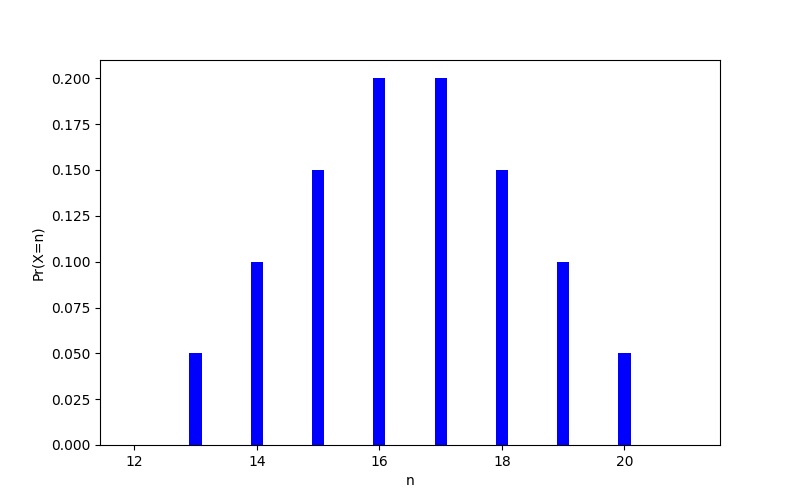
\includegraphics[width=\columnwidth]{solutions/ee/2015/2/Figure_1.png}
    \caption{Probability mass function of X}
    \label{ee2015-2:Figure_1}
\end{figure}
\begin{align}
    p_x(n) = 
    \begin{cases}
    0 & n \leq 12\\
    \frac{n-12}{20}  & 13 \leq n \leq 16\\
    \frac{21-n}{20}  & 17 \leq n \leq 20\\
    0 & n>20
    \end{cases}\label{ee2015-2:6}
\end{align}
Required probability is the probability of the sum of numbers selected from the sets, one from each set to be 16.\\
Therefore from \eqref{ee2015-2:6},
\begin{align}
    p_X(16) &= \left(\frac{16-12}{20}\right)\\
    \implies p_X(16) &= \frac{4}{20}\\
    \implies\pr{X_1+X_2=16} &= \frac{1}{5} \\
    \therefore \pr{X_1+X_2=16}  &= 0.2
\end{align}


%
\item Let X and Y be two statistically independent random variables uniformly distributed in the range (-1, 1) and (-2, 1) respectively. Let $Z = X +Y$ , then the probability that $[Z \leq -2]$ is\\
(A) 0\\
(B) $\frac{1}{6}$\\
(C) $\frac{1}{3}$\\
(D) $\frac{1}{12}$
%\\
%\solution
%\input{solutions/ec/2003/61/Assignment_4.tex}

%
\item Two die are thrown. What is the probability that sum of numbers on the two dice is eight \\
\begin{enumerate}[label=(\alph*)]
\item $\frac{5}{36}$\\
\item $\frac{5}{18}$ \\
\item$\frac{1}{4}$\\
\item$\frac{1}{3}$
\end{enumerate}
%
%
\solution
Let $X$ be a discrete random variable which denotes the sum obtained on two dice and $X_{1} \in \{1,6\}$ be a discrete random variable denoting the outcome on a single die.
\begin{align}
\pr{X=n}=
\begin{cases}
 0 , &\text{if } n < 1 \\
 \frac{n-1}{36} , &\text{if } 1 \leq n-1 \leq 6\\
 \frac{13-n}{26} , &\text{if } 1 < n-6 \leq 6\\
 0 , &\text{if } n > 12 \label{me2002-1.1:1.0.1}
\end{cases}
\end{align}
\begin{align}
    \text{Required probability}  = \pr{X=8}  \notag 
\end{align}
\begin{align}
  \text{So, from \eqref{me2002-1.1:1.0.1},}  \pr{X=8}= \frac{5}{36} \notag
\end{align}

\item Four fair six-sided dice are rolled.The probability that sum of results being 22 is $\frac{X}{1296}$.the value of X is
%
\solution



Let X and Y be a random variable which takes values from set A and B respectively.We want to calculate Pr(X+Y=16)
\begin{equation}
  p_X(n)=\begin{cases}
    \dfrac{1}{4}, & \text{if } 2\leq n\leq 5.\\
    0, & \text{otherwise}.
  \end{cases}
\end{equation}
\begin{equation}
  p_Y(n)=\begin{cases}
    \dfrac{1}{5}, & \text{if } 11\leq n\leq 15.\\
    0, & \text{otherwise}.
  \end{cases}
\end{equation}
\begin{align}
&p_z(n) = \Pr(X+Y = n) = \Pr(Y=n-X)\\
&p_z(n) = \sum_k p_x(k)p_y(n-k) = p_x(n) * p_y(n)\\
&p_z(n) = \frac{1}{4} \sum_{k=2}^5 p_y(n-k)=\frac{1}{4}\sum_{k=n-5}^{n-2} p_y(k)
\end{align}
\begin{equation}
  p_z(n)=\begin{cases}
  &0 , n < 13\\
  &\dfrac{1}{20}\times (n-12) ,13 \leq n < 16\vspace{0.2cm}\\
  &\dfrac{1}{20} \times 4 , 16 \leq n \leq 17\vspace{0.2cm}\\
  &\dfrac{21-n}{20} , 18 \leq n \leq 20\vspace{0.2cm}\\
  & 0 ,n > 20
  \end{cases}
\end{equation}
\begin{align}
\therefore p_z(16) = \frac{1}{5}
\end{align}
\begin{figure}[h]
    \centering
    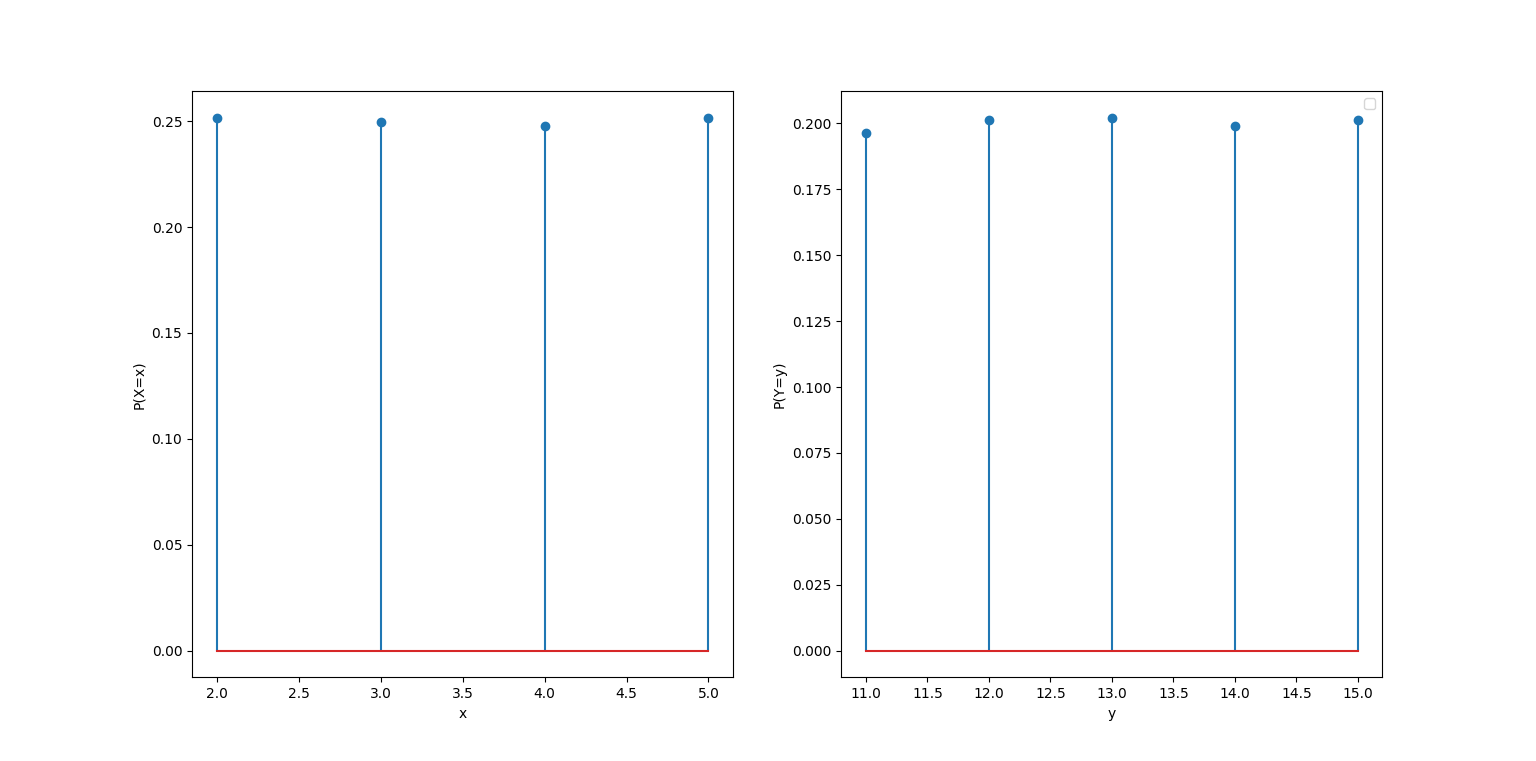
\includegraphics[width=\columnwidth]{solutions/cs/2015/3/figures/assignment4_plot2.png}
\end{figure}
\begin{figure}[h]
    \centering
    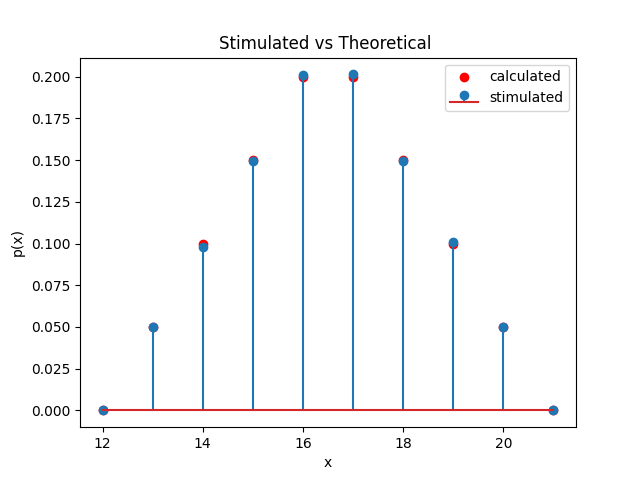
\includegraphics[width=\columnwidth]{solutions/cs/2015/3/figures/assignment4_plot1.png}
\end{figure}



%
\item Let $X$ and $Y$ be two statistically independent random variables uniformly
distributed in the ranges $(-1,1)$ and $(-2,1)$ respectively. Let $Z = X + Y.$ then the probability that $[Z\leq-2]$ is
\begin{enumerate}[label=\alph*)]
\item zero
\item $\frac{1}{6}$
\item $\frac{1}{3}$
\item $\frac{1}{12}$
\end{enumerate}
%
\solution

The pdf of $Z(=X+Y)$ will be convolution of pdf of $X$ and pdf of $Y$ as shown below.
\begin{align}
f_{x}( x)\times f_{y}(y)=f_{z}(z)
\end{align}
\tikzset{every picture/.style={line width=0.5pt}} %set default line width to 0.75pt        
\begin{tikzpicture}[x=0.45pt,y=0.5pt,yscale=-1,xscale=1]
%uncomment if require: \path (0,300); %set diagram left start at 0, and has height of 300
%Straight Lines [id:da7994322016020907] 
\draw [line width=0.75]    (65.3,280.6) -- (580.3,280.6) ;
%Straight Lines [id:da6298726397789813] 
\draw [line width=0.75]    (321.8,68.4) -- (322.8,280.6) ;
%Shape: Right Angle [id:dp8023791863547924] 
\draw  [color={rgb, 255:red, 0; green, 0; blue, 0 }  ,draw opacity=1 ][line width=1.5]  (254.8,168.6) -- (389.8,168.6) -- (389.8,279) ;
%Straight Lines [id:da07001326664875096] 
\draw [line width=1.5]    (254.8,168.6) -- (254.8,279) ;
% Text Node
\draw (403,152.4) node [anchor=north west][inner sep=0.75pt]    {$\dfrac{1}{2}$};
% Text Node
\draw (240,285.4) node [anchor=north west][inner sep=0.75pt]    {$-1$};
% Text Node
\draw (385,282.4) node [anchor=north west][inner sep=0.75pt]    {$1$};
% Text Node
\draw (318,283.4) node [anchor=north west][inner sep=0.75pt]    {$0$};
% Text Node
\draw (303,44.4) node [anchor=north west][inner sep=0.75pt]    {$f_{x}( x)$};
% Text Node
\draw (590,269.4) node [anchor=north west][inner sep=0.75pt]    {$x$};
\end{tikzpicture}
\tikzset{every picture/.style={line width=0.5pt}} %set default line width to 0.75pt        
\begin{tikzpicture}[x=0.45pt,y=0.5pt,yscale=-1,xscale=1]
%uncomment if require: \path (0,300); %set diagram left start at 0, and has height of 300
%Straight Lines [id:da7994322016020907] 
\draw [line width=0.75]    (65.3,280.6) -- (580.3,280.6) ;
%Straight Lines [id:da6298726397789813] 
\draw [line width=0.75]    (321.8,68.4) -- (322.8,280.6) ;
%Shape: Right Angle [id:dp8023791863547924] 
\draw  [color={rgb, 255:red, 0; green, 0; blue, 0 }  ,draw opacity=1 ][line width=1.5]  (267.8,168.6) -- (389.8,168.6) -- (389.8,279) ;
%Straight Lines [id:da07001326664875096] 
\draw [line width=1.5]    (267.8,168.6) -- (189.8,169.4) -- (189.8,280) ;
% Text Node
\draw (403,152.4) node [anchor=north west][inner sep=0.75pt]    {$\dfrac{1}{3}$};
% Text Node
\draw (240,282.4) node [anchor=north west][inner sep=0.75pt]    {$-1$};
% Text Node
\draw (385,282.4) node [anchor=north west][inner sep=0.75pt]    {$1$};
% Text Node
\draw (318,283.4) node [anchor=north west][inner sep=0.75pt]    {$0$};
% Text Node
\draw (303,44.4) node [anchor=north west][inner sep=0.75pt]    {$f_{y}( y)$};
% Text Node
\draw (590,269.4) node [anchor=north west][inner sep=0.75pt]    {$y$};
% Text Node
\draw (175,280.4) node [anchor=north west][inner sep=0.75pt]    {$-2$};
\end{tikzpicture}
\tikzset{every picture/.style={line width=0.5pt}} %set default line width to 0.75pt        
\begin{tikzpicture}[x=0.45pt,y=0.5pt,yscale=-1,xscale=1]
%uncomment if require: \path (0,300); %set diagram left start at 0, and has height of 300
%Straight Lines [id:da7994322016020907] 
\draw [line width=0.75]    (65.3,280.6) -- (580.3,280.6) ;
%Straight Lines [id:da6298726397789813] 
\draw [line width=0.75]    (321.8,68.4) -- (322.8,280.6) ;
%Straight Lines [id:da3048610517318646] 
\draw [line width=1.5]    (249.8,174.8) -- (322.3,174.5) ;
%Straight Lines [id:da21348606992409946] 
\draw [line width=1.5]    (249.8,174.8) -- (126.8,280.8) ;
%Straight Lines [id:da9537386999126634] 
\draw [line width=1.5]    (322.3,174.5) -- (460.8,279.8) ;
%Straight Lines [id:da7472472432945507] 
\draw  [dash pattern={on 0.84pt off 2.51pt}]  (391.55,227.15) -- (188.3,227.8) ;
%Straight Lines [id:da7478392311577124] 
\draw  [dash pattern={on 0.84pt off 2.51pt}]  (188,281) -- (188.3,227.8) ;
%Straight Lines [id:da11363593871174427] 
\draw  [dash pattern={on 0.84pt off 2.51pt}]  (253.8,278) -- (254.8,228) ;
%Straight Lines [id:da30914849700103675] 
\draw  [dash pattern={on 0.84pt off 2.51pt}]  (390.8,278) -- (391.55,227.15) ;
% Text Node
\draw (350,153.4) node [anchor=north west][inner sep=0.75pt]    {$\dfrac{1}{3}$};
% Text Node
\draw (241,282.4) node [anchor=north west][inner sep=0.75pt]    {$-1$};
% Text Node
\draw (385,282.4) node [anchor=north west][inner sep=0.75pt]    {$1$};
% Text Node
\draw (318,283.4) node [anchor=north west][inner sep=0.75pt]    {$0$};
% Text Node
\draw (271,50.4) node [anchor=north west][inner sep=0.75pt]    {$f_{Z}( z) =f_{x}( \ x) \times \ f_{y} y)$};
% Text Node
\draw (175,280.4) node [anchor=north west][inner sep=0.75pt]    {$-2$};
% Text Node
\draw (114,282.4) node [anchor=north west][inner sep=0.75pt]    {$-3$};
% Text Node
\draw (455,282.4) node [anchor=north west][inner sep=0.75pt]    {$2$};
% Text Node
\draw (586,271.4) node [anchor=north west][inner sep=0.75pt]    {$z$};
% Text Node
\draw (415,198.4) node [anchor=north west][inner sep=0.75pt]    {$\dfrac{1}{6}$};
\end{tikzpicture}
Now
\begin{align}
\pr{Z \leq z} &=\int_{-\infty}^{z} f_{Z}(z) d z \\
\pr{Z \leq-2} &=\int_{-\infty}^{-2} f_{Z}(z) d z \\
&=\text {Area }[z \leq-2] \\
&=\frac{1}{2} \times \frac{1}{6} \times 1=\frac{1}{12}
\end{align}
Hence $(\mathrm{D})$ is correct option.

%
\item A single die is thrown twice. What is the probability that the sum is neither 8 or 9?
    \begin{enumerate}[label=(\alph*)]
        \item \large$\frac{1}{9}$
        \item \large$\frac{5}{36}$
        \item \large$\frac{1}{4}$
        \item \large$\frac{3}{4}$
    \end{enumerate}
%
\solution

Let $X \in \{0,1\}$ be the random variable, where X=0 represents that we get sum to be 8 or 9 and X=1 represents that we get sum between 2 and 12 except 8 and 9.\\
Total number of possible outcomes is :
\begin{equation}
    N = {\comb{6}{1}}\times{\comb{6}{1}} = 36
\end{equation}
 
Probability that the sum is neither 8 or 9 
\begin{equation}\label{me2005-38:eq:2}
  \pr{X=1} = 1-\pr{X=0}
\end{equation}
 Only 9 outcomes are favourable to the occurrence of X=0 .\\
Probability of getting sum 8 or 9 is :
\begin{equation}
    \pr{X=0} = \frac{9}{36}
             = \frac{1}{4}
\end{equation}
Substituting value in \eqref{me2005-38:eq:2} , we get
\begin{equation}
 \pr{X=1} = 1- \frac{1}{4}
          = \frac{3}{4}   
\end{equation}
Hence, the correct option is (d) \large$\frac{3}{4}$
%

\end{enumerate}